\subsection{\'Etapes de validation}
\begin{frame}{Premiers outils de v\'erification}
  \begin{block}{}
    \begin{itemize}
      \item Validation des politiques basiques
      \item Validation du comportement inclusif
      \item Utilisation de PAPI
    \end{itemize}
  \end{block}
        
\end{frame}

\begin{frame}{Benchmarks basiques}
\begin{figure}[H]
   \begin{minipage}[l]{.46\textwidth}
     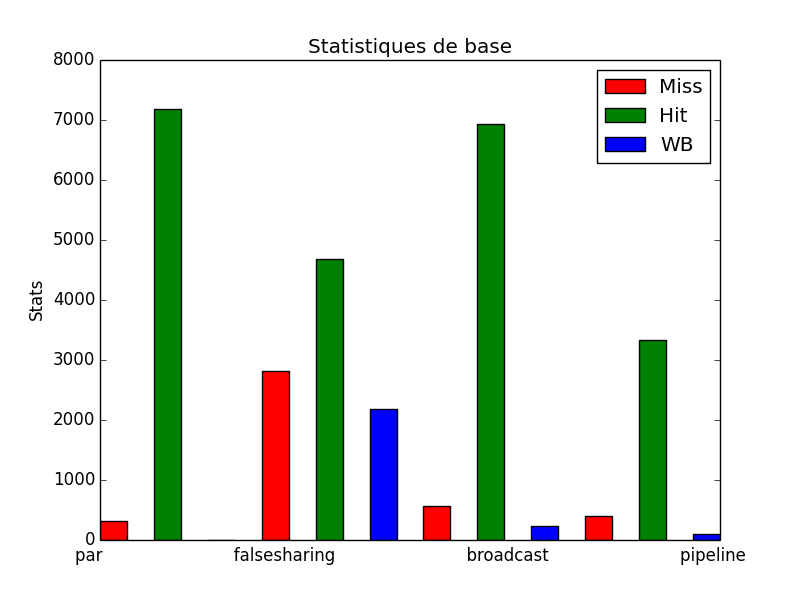
\includegraphics[scale=0.22]{images/stats_L1.png}
   \end{minipage} \hfill
   \begin{minipage}[r]{.46\textwidth}
     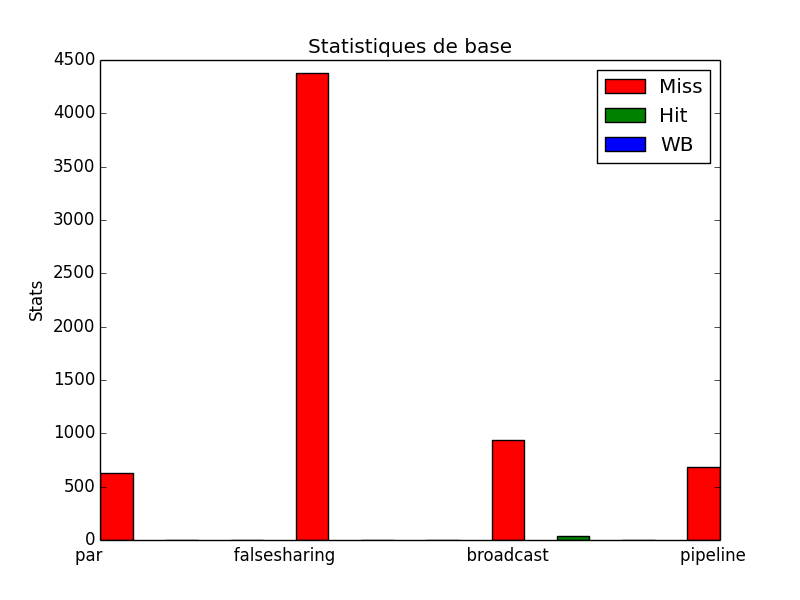
\includegraphics[scale=0.22]{images/stats_L2.png}
   \end{minipage}
\end{figure}

\begin{figure}[t!]
  \begin{minipage}[l]{.46\textwidth}
    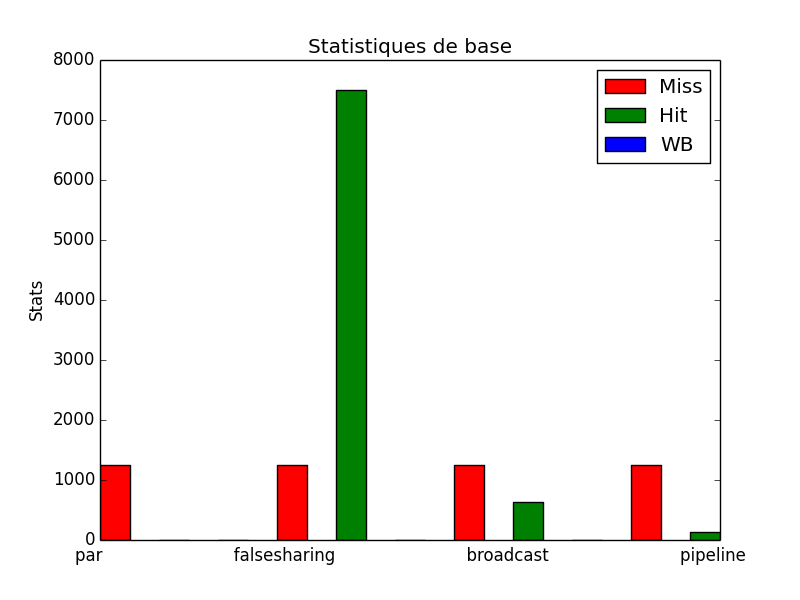
\includegraphics[scale=0.22]{images/stats_L3.png}
  \end{minipage} \hfill
   \begin{minipage}[r]{.46\textwidth}
     Gauche: L1 \\
     Droite: L2 \\
     Bas: L3
   \end{minipage}
\end{figure}
\end{frame}

\begin{frame}{Benchmarks avanc\'es}
\begin{figure}[H]
   \begin{minipage}[l]{.46\textwidth}
     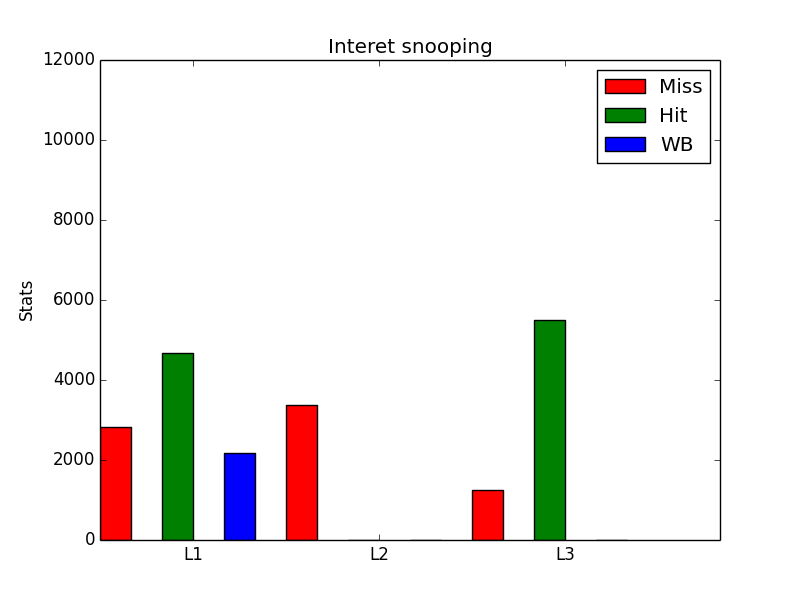
\includegraphics[scale=0.22]{images/stats_falsesharing_snooping.png}
     \caption{Avec \emph{snooping}}
   \end{minipage} \hfill
   \begin{minipage}[r]{.46\textwidth}
     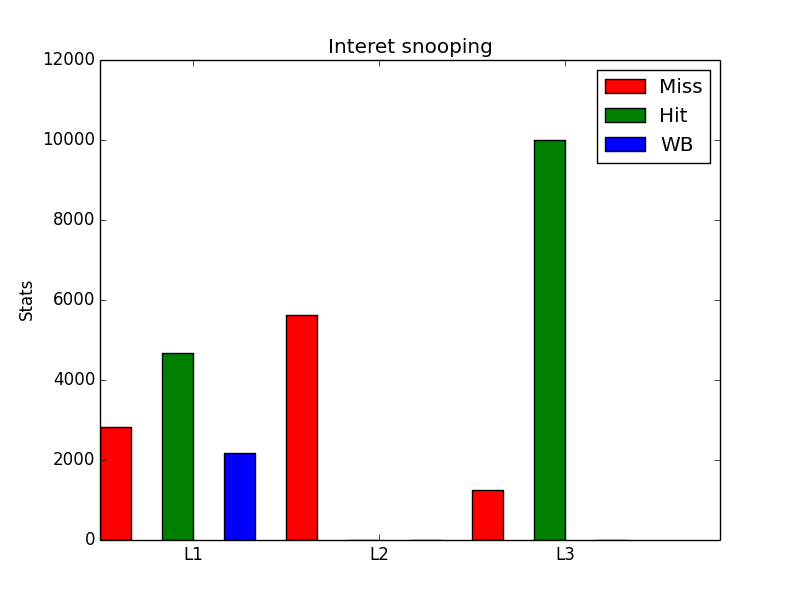
\includegraphics[scale=0.22]{images/stats_falsesharing_no_snooping.png}
     \caption{Sans \emph{snooping}}
   \end{minipage}
\end{figure}
  \begin{block}{Autres benchmarks}
    \begin{itemize}
      \item \emph{Directory manager}
      \item Politiques de coh\'erence MSI \emph{vs} MESI
      \item Scalabilit\'e
    \end{itemize}
  \end{block}
\end{frame}

\subsection{Limites \`a  propos de la simulation des caches}
\begin{frame}
  \begin{block}{Probl\`emes li\'es aux architectures multi-c{\oe}ur}
    \begin{itemize}
      \item \emph{prefetching}
      \item synchronisations
      \item changements de contextes 
      \item optimisations du compilateur
    \end{itemize}
  \end{block}
  \begin{block}{Limites de Cassis}
    \begin{itemize}
      \item bande passante non mod\'elis\'ee
      \item \emph{directory manager} basiquement mod\'elis\'es
      \item statistiques non calibr\'ees avec des benchmarks classiques
      \item utilisation de m\'etriques non usuelles
    \end{itemize}
  \end{block}
\end{frame}


\section*{Conclusion}
\begin{frame}
  \begin{block}{Objectifs atteints}
    \begin{itemize}
      \item Cahier des charges respect\'e
      \item Param\'etrisation compl\`ete
    \end{itemize}
  \end{block}

  \begin{block}{\'Evolution possible}
    \begin{itemize}
      \item Couplage avec un simulateur \emph{on-line}?
      \item Utilisation de benchmarks pour calibrer les r\'esultats?
      \item Annotation du code source
    \end{itemize}
  \end{block}
\end{frame}

\begin{frame}
\begin{center}
  Merci de votre attention
  \begin{center}
  
\includegraphics[scale=.5]{images/cassis.png}
  \end{center}
\end{center}
\end{frame}
